\section{Satz von Gauss}
Sei $R$ ein faktorieller Ring, $K= \Quot(R)$ und $p \in R$ prim.

\begin{remark}
	\textbf{Ziel:} $R$ faktoriell $\Rightarrow R[x]$ faktoriell.\\
	Dafür studieren wir die folgenden Ringe:
	\begin{center}
		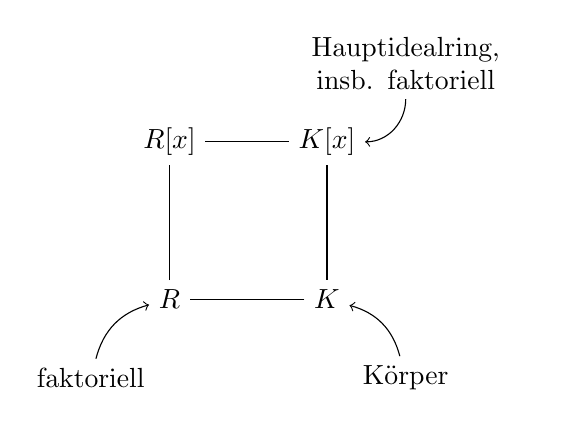
\begin{tikzpicture}
			\node at (0,0) (Rx) {$R[x]$};
			\node at (2,0) (Kx) {$K[x]$};
			\node at (0,-2) (R) {$R$};
			\node at (2,-2) (K) {$K$};
			
			\draw (Rx) -- (Kx) -- (K) -- (R) -- (Rx);
			
			\node at (-1,-3) (f) {faktoriell};
			\draw[->,bend left] (f) to (R);
			
			\node at (3,-3) (k) {Körper};
			\draw[->,bend right] (k) to (K);
			
			\node[text width=3cm,align=center] at (3,1) (h) {Hauptidealring, insb. faktoriell};
			\draw[->,out=270] (h) to [in=0] (Kx);
		\end{tikzpicture}
	\end{center}
\end{remark}

\begin{definition}
	\proplbl{2_6_2}
	Für $f = \sum_{i \ge 0} a_i x^i \in K[x]$. Sei $v_p(f) := \min_{i \ge 0} v_p(a_i) \in \whole \cup \{\infty\}$.
\end{definition}

\begin{remark}
	\proplbl{2_6_3}
	Seien $f,g \in K[x]$.
	\begin{enumerate}[label=(\alph*)]
		\item $f \in R[x] \Leftrightarrow v_p(f) \ge 0$ für alle $p \in R$ prim.
		\item $v_p(f+g) \ge \min\{v_p(f), v_p(g)\}$ (betrachte koeffizientenweise)
	\end{enumerate}
\end{remark}

\begin{definition}[Koeffizientenreduktion]
	\proplbl{2_6_4}
	Der Homomorphismus
	\begin{align}
	\pi_{(p)}: \begin{cases}
	R &\to \lnkset{R}{(p)} \\
	x &\mapsto \overline{x} := x + (p)
	\end{cases}\notag
	\end{align}
	setzt sich nach \propref{2_1_12} zu einem Homomorphismus
	\begin{align}
	\begin{cases}
		R[x] &\to \left(\lnkset{R}{(p)}\right)[x]\\
		f=\sum_{i \ge 0} a_i x^i &\mapsto \overline{f} := \sum_{i \ge 0} \overline{a}_i x^i
	\end{cases}\notag
	\end{align}
	fort, genannt \begriff{Koeffizientenreduktion}. Dabei ist $\overline{f} = 0 \Leftrightarrow \overline{a}_i = 0 \quad\forall i \Leftrightarrow v_p(a_i) \ge 1 \quad\forall i \Leftrightarrow v_p(f) > 0$.
\end{definition}

\begin{proposition}[Lemma von \person{Gauss}]
	\proplbl{2_6_5}
	Für $f,g \in K[x]$ ist $v_p(fg) = v_p(f)+v_p(g)$.
\end{proposition}

\begin{proof}
	o.B.d.A. seien $f,g \neq 0$. Für $h= \sum_{i \ge 0} a_i x^i \in K[x]$, $c \in K^{\times}$ ist $v_p(c\cdot h) = \min v_p(c\cdot a_i) = v_p(c) + v_p(f)$. Wir können deshalb ohne Einschränkung $f$ und $g$ mit $c \in K^{\times}$ multiplizieren. \\
	$\Rightarrow f,g \in R[x] \text{ z.B. multiplikation mit Produkt der Nenner}$ \\
	$\Rightarrow\text{ohne Einschränkung } v_p(f),v_p(g) = 0$ \\
	Dann ist $\overline{f}, \overline{g} \neq 0$. Wegen $p$ prim ist $\lnkset{R}{(p)}$ nullteilerfrei und weiter $\left(\lnkset{R}{(p)} \right) [x]$ nullteilerfrei. Somit folgt $\overline{fg} \overset{\propref{2_6_4}}{=} \overline{f}\cdot\overline{g} \neq 0$, das heißt $v_p(fg) = 0 = v_p(f)+v_p(g)$.
\end{proof}

\begin{conclusion}
	\proplbl{2_6_6}
	Ist $f \in R[x]$ normiert und $f=gh$ mit $g,h \in K[x]$ normiert, so sind $g,h \in R[x]$.
\end{conclusion}

\begin{proof}
	Sei $p \in R$ prim. Da $f \in R[x]$ ist $v_p(f) \ge 0$. Da $f,g,h$ normiert sind ist $v_p(f), v_p(h), v_p(g) \le 0$ \\
	$\Rightarrow 0 = v_p(f) = v_p(gh) = \underbrace{v_p(g)}_{\le 0} + \underbrace{v_p(h)}_{\le 0}$ \\
	$\Rightarrow v_p(g), v_p(h) = 0$ \\
	Somit folgt $g,h \in R[x]$ (vgl. \propref{2_6_3}a).
\end{proof}

\begin{conclusion}
	Sei $f \in R[x]$ normiert. Ist $a \in K$ mit $f(a)=0$, so ist $a \in R$.
\end{conclusion}

\begin{proof}
	Sei $f(a)=0$.\\
	$Rightarrow f(x) = f(x \cdot a)g(x) \text{ mit } g \in K[x] \text{ normiert}$ \\
	$\overset{\propref{2_6_6}}{\Rightarrow} x - a \in R[x]\text{, das heißt } a \in R.$
\end{proof}

\begin{definition}[Inhalt, primitiv]
	Sei $f = \sum_{i =0}^{n} a_i x^i \in R[x]$.
	\begin{enumerate}[label=(\alph*)]
		\item $I(f) = \ggT(a_0,\dots,a_n)$, der \begriff{Inhalt} von $f$.
		\item $f$ \begriff{primitiv} $:\Leftrightarrow I(f) \sim 1$.
	\end{enumerate}
\end{definition}

\begin{*anmerkung}
	Sei $f(x)=x^2+5x+2$. Dann ist $p=5$ und $q=2$. Dann
	\begin{align}
		x_{1/2} &= -\frac{p}{2}\pm \sqrt{\left(\frac{p}{2}\right)^2-q} \notag \\
		&= -\frac{5}{2} \pm \sqrt{\frac{25}{4}-\frac{8}{4}} \notag
	\end{align}
\end{*anmerkung}

\begin{remark}
	\proplbl{2_6_9}
	\begin{enumerate}[label=(\alph*)]
		\item $I(f)$ ist nur bis auf Einheiten bestimmt. Ist $\mathbb{P}$ Vertretersystem der Primelemente von $R$ modulo Assoziiertheit, so ist
		\begin{align}
			I(f) \sim \prod_{p \in \mathbb{P}} p^{v_p(f)}\notag
		\end{align}
		\item Umformulierungen des Lemma von \person{Gauss}: $I(fg) = I(f)\cdot I(g)$.
		\item Zu $f \in R[x]$ existiert $c \in R$, $f_0 \in R[x]$ primitiv mit $f = c\cdot f_0$, nämlich $c = I(f)$. Zu $f \in K[x]$ existiert $c \in K$, $f_0 \in R[x]$ primitiv mit $f = c \cdot f_0$ (erst mit Produkt den Nenner multiplizieren).
	\end{enumerate}
\end{remark}

\begin{theorem}[Satz von \person{Gauss}]
	\proplbl{2_6_10}
	Sei $R$ faktorieller Ring und $K = \Quot(R)$. Dann ist auch $R[x]$ faktoriell. Ein $f \in R[x]$ ist genau dann prim, wenn
	\begin{enumerate}[label=(\alph*)]
	\item $f$ ist ein Primelement von $R$ \textbf{oder}
	\item $f$ ist primitiv und ist ein Primelement in $K[x]$.
	\end{enumerate}
\end{theorem}

\begin{proof}
	Sei $0 \neq f \in R[x]\setminus R^{\times}$, $g,h \in R[x]$.
	\begin{itemize}
	\item $f$ vom Typ (a) $\Rightarrow f$ prim in $R[x]:$ Sei $f = p \in R$ prim in $R$.
	\begin{align}
	p \mid gh &\Rightarrow 0 < v_p(gh) \overset{\propref{2_6_5}}{=} \underbrace{v_p(g)}_{\ge 0} + \underbrace{v_p(h)}_{\ge 0}\notag \\
	&\Rightarrow \text{ ohne Einschränkung } v_p(g) > 0\text{, das heißt }p \mid g. \notag
	\end{align}
	\item $f$ vom Typ (b) $\Rightarrow f$ prim in $R[x]$:
	\begin{align}
		f \mid gh \text{ in } R[x] &\Rightarrow f\mid gh \text{ in } K[x]\notag \\
		&\xRightarrow[\text{in } K\lbrack x\rbrack]{f \text{ prim}}\text{ ohne Einschränkung } f \mid g \text{ in } K[x]\text{, das heißt existiert } q \in K[x] \text{ mit } g = q\cdot f.\notag
	\end{align}
	Für $p \in R$ prim ist:
	\begin{align}
		0\le v_p(g) = v_p(q) + \underbrace{v_p(f)}_{=0,\, f \text{ primitiv}} = v_p(q). \notag
	\end{align}
	Somit folgt $q \in R[x]$ und damit $f\mid g$ in $R[x]$.
	\item $f$ ist Produkt von Elementen vom Typ (a) oder Typ (b). Schreibe $f = c f_0, c \in R, f_0 \in R[x]$ primitiv (\propref{2_6_9}c)). $c$ ist Produkt von Elementen vom Typ (a) (oder $c \in R^{\times}$):
	Da $K[x]$ faktoriell ist, ist $f_0 = c_0 g_1\cdots g_n$, $c \in K^{\times}, g_1, \dots, g_n \in K[x]$ prim. Nach $\propref{2_6_9}c)$ ist ohne Einschränkung  $g_1,\dots,g_n \in R[x]$ primitiv, also vom Typ (b).
	Für $p \in R$ prim ist
	\begin{align}
	0 = v_p(f_0) = v_p(c_0) + \underbrace{v_p(g_1)}_{=0} +\cdots + \underbrace{v_p(g_n)}_{=0} &= v_p(c_0)\notag \\
	&\Rightarrow c_0 \in R^{\times}.\notag
	\end{align}
	\item Somit ist $R[x]$ faktoriell. Ist $f \in R[x]$ prim, so ist $f = f_1\cdots f_n$ mit $f_i$ vom Typ (a) oder Typ (b): \\
	$\Rightarrow n =1$, somit $f=f_1$ vom Typ (a) oder Typ (b).
	\begin{itemize}
		\item Ist $f \in R[x]$ vom Typ (a), so ist $f \not \in R[x]^{\times} = R^{\times}$ und somit prim in $R[x]$.
		\item Ist $f \in R[x]$ vom Typ (b), so ist $f \not \in K[x]^{\times}$, insbesondere $f \not \in R[x]^{\times}$, somit $f$ prim in $R[x]$.
	\end{itemize}
	\end{itemize}
\end{proof}

\begin{example}
	Für $F$ Körper ist $F[x_1,\dots,x_n]$ faktoriell, aber für $n > 1$ kein Hauptidealring (vgl. V108)!
\end{example}